\documentclass[tikz,border=3pt]{standalone}
\usepackage[utf8]{inputenc}
\usepackage[T1]{fontenc}
\usepackage{lmodern}
\renewcommand{\familydefault}{\sfdefault}
\usepackage{sansmath}\sansmath
\usepackage{chemfig}
\usepackage{pgfplots}\pgfplotsset{compat=1.18,/pgf/number format/use comma,/pgf/number format/1000 sep={.}}
\usetikzlibrary{arrows.meta,calc,positioning,decorations.pathmorphing,patterns}
% paleta del sitio
\definecolor{nar}{HTML}{E8680C}\definecolor{narc}{HTML}{FFB35C}\definecolor{hielo}{HTML}{FFF3E8}
\definecolor{tinta}{HTML}{1D1D1F}\definecolor{gris}{HTML}{6E6E73}\definecolor{lila}{HTML}{7C5CF0}
\definecolor{azul}{HTML}{2F6FD6}\definecolor{menta}{HTML}{17A673}\definecolor{coral}{HTML}{E8342A}
\tikzset{cel/.style={draw=gris,fill=hielo,line width=0.9pt},nuc/.style={draw=gris!70,line width=0.6pt},
fib/.style={gris!55,line width=0.35pt},eti/.style={font=\footnotesize,text=tinta,align=center},
num/.style={circle,draw=nar,fill=white,text=nar,font=\small\bfseries,inner sep=1.2pt,minimum size=13pt},
fl/.style={-{Stealth[length=2.6mm]},gris,line width=0.9pt}}
\begin{document}
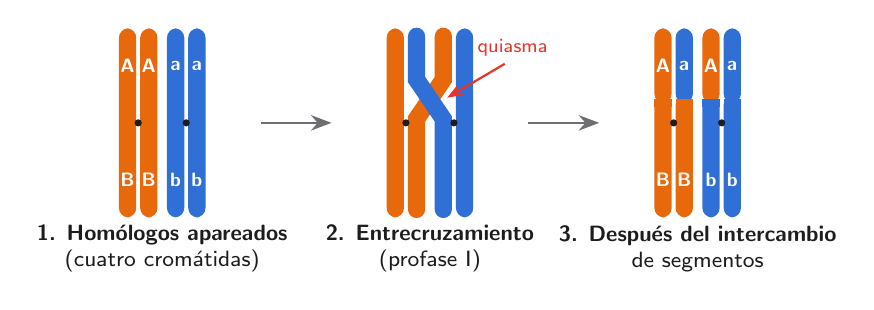
\begin{tikzpicture}[font=\small]
\fill[nar,rounded corners=1.2mm] (-0.55,-1.2) rectangle (-0.33,1.2);
\node[text=white,font=\scriptsize\bfseries] at (-0.44,0.72) {A};
\node[text=white,font=\scriptsize\bfseries] at (-0.44,-0.72) {B};
\fill[nar,rounded corners=1.2mm] (-0.28,-1.2) rectangle (-0.06,1.2);
\node[text=white,font=\scriptsize\bfseries] at (-0.17,0.72) {A};
\node[text=white,font=\scriptsize\bfseries] at (-0.17,-0.72) {B};
\fill[azul,rounded corners=1.2mm] (0.06,-1.2) rectangle (0.28,1.2);
\node[text=white,font=\scriptsize\bfseries] at (0.17,0.72) {a};
\node[text=white,font=\scriptsize\bfseries] at (0.17,-0.72) {b};
\fill[azul,rounded corners=1.2mm] (0.33,-1.2) rectangle (0.55,1.2);
\node[text=white,font=\scriptsize\bfseries] at (0.44,0.72) {a};
\node[text=white,font=\scriptsize\bfseries] at (0.44,-0.72) {b};
\fill[tinta] (-0.305,0) circle (1.3pt);
\fill[tinta] (0.305,0) circle (1.3pt);
\fill[nar,rounded corners=1.2mm] (2.85,-1.2) rectangle (3.07,1.2);
\fill[azul,rounded corners=1.2mm] (3.73,-1.2) rectangle (3.95,1.2);
\draw[nar,line width=6.2pt,line cap=round] (3.23,-1.1)--(3.23,0.05)--(3.57,0.55)--(3.57,1.1);
\draw[azul,line width=6.2pt,line cap=round] (3.57,-1.1)--(3.57,0.05)--(3.23,0.55)--(3.23,1.1);
\fill[tinta] (3.095,0) circle (1.3pt);
\fill[tinta] (3.705,0) circle (1.3pt);
\draw[coral,thick,-{Stealth[length=2mm]}] (4.35,0.75)--(3.62,0.32);\node[eti,font=\scriptsize,text=coral] at (4.45,0.95) {quiasma};
\fill[nar,rounded corners=1.2mm] (6.25,-1.2) rectangle (6.47,0.35);
\fill[nar,rounded corners=1.2mm] (6.25,0.25) rectangle (6.47,1.2);
\fill[nar] (6.25,0.2) rectangle (6.47,0.3);
\node[text=white,font=\scriptsize\bfseries] at (6.36,0.72) {A};
\node[text=white,font=\scriptsize\bfseries] at (6.36,-0.72) {B};
\fill[nar,rounded corners=1.2mm] (6.52,-1.2) rectangle (6.74,0.35);
\fill[azul,rounded corners=1.2mm] (6.52,0.25) rectangle (6.74,1.2);
\fill[nar] (6.52,0.2) rectangle (6.74,0.3);
\node[text=white,font=\scriptsize\bfseries] at (6.63,0.72) {a};
\node[text=white,font=\scriptsize\bfseries] at (6.63,-0.72) {B};
\fill[azul,rounded corners=1.2mm] (6.86,-1.2) rectangle (7.08,0.35);
\fill[nar,rounded corners=1.2mm] (6.86,0.25) rectangle (7.08,1.2);
\fill[azul] (6.86,0.2) rectangle (7.08,0.3);
\node[text=white,font=\scriptsize\bfseries] at (6.97,0.72) {A};
\node[text=white,font=\scriptsize\bfseries] at (6.97,-0.72) {b};
\fill[azul,rounded corners=1.2mm] (7.13,-1.2) rectangle (7.35,0.35);
\fill[azul,rounded corners=1.2mm] (7.13,0.25) rectangle (7.35,1.2);
\fill[azul] (7.13,0.2) rectangle (7.35,0.3);
\node[text=white,font=\scriptsize\bfseries] at (7.24,0.72) {a};
\node[text=white,font=\scriptsize\bfseries] at (7.24,-0.72) {b};
\fill[tinta] (6.495,0) circle (1.3pt);
\fill[tinta] (7.105,0) circle (1.3pt);
\draw[fl] (1.25,0)--(2.15,0);
\draw[fl] (4.65,0)--(5.55,0);
\node[eti] at (0,-1.6) {\textbf{1. Homólogos apareados}\\(cuatro cromátidas)};
\node[eti] at (3.4,-1.6) {\textbf{2. Entrecruzamiento}\\(profase I)};
\node[eti] at (6.8,-1.6) {\textbf{3. Después del intercambio}\\de segmentos};
\end{tikzpicture}
\end{document}
